%! Author = fatihergin
%! Date = 2020-05-03

\section{Artificial Neural Networks}

    Artificial Neural Networks (ANNs) are a category of supervised machine learning algorithms whose design has been inspired by the neurophysiological workings of the human brain \cite{hill1994artificial}.
    These networks consist of several layers mainly first layer, last layer and middle layer(s).
    The first layer is known as the input layer, middle layer which is called as hidden layer and the last layer is the output layer where each layer has several artificial neurons.
    An example of ANN with a single hidden layer can be seen at Figure~\ref{fig:sample-ann}.
    The most common layer organization is the fully connected layer, where each neuron is fully paired with adjacent neurons.

    An ANN transform the inputs into outputs using the activation function, bias and weights.
    To explain, the sum of inputs is multiplied by weights; the deviation is added and the result is passed through the activation function which is selected by purpose.
    Deciding whether the neuron is active is determined by the activation function.

    \begin{figure}
    \centerline{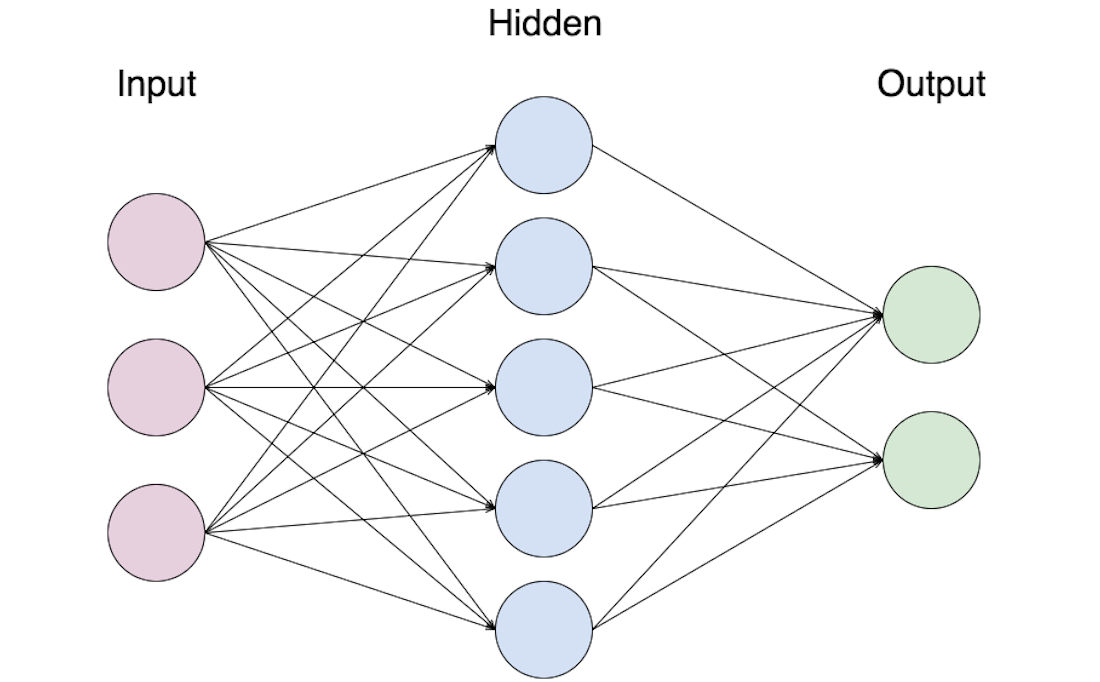
\includegraphics[width=1\columnwidth]{03-neural-networks-in-tumor-detection/figures/sample-ann.png}}
    \caption{Sample ANN with three inputs, one hidden layer, and one output }
    \label{fig:sample-ann}
\end{figure}

    During the training, training samples are sent one by one through the network.
    The output value is calculated for each sample sent.
    Output values are compared to the target with the help of a loss function to minimize the error rate.
    At the backpropagation step, the network is updated by propagating errors backwards through the network \cite{lecun1988theoretical}.

    \subsection{Weight Update}

        Gradient descent is used to minimize the loss function of the neural network.
        The first-order derivative of the loss function, namely gradient is computed at the current point and it is used to increase the slope in the opposite direction by moving in by the value of self.
        These two steps are applied to the weights in each cycle.
        Batch gradient descent (BGD), stochastic gradient descent (SGD), and mini-batch gradient descent are some of the commonly used weight update methods.
        In SGD, the training samples are randomly shuffled, to put it another way, the weights are updated after each training sample \cite{bottou2010large}.
        On the other hand, all the training samples are used at weight update in batch gradient descent.
        SGD requires more calculations than batch gradient descent and it is more sensitive than the other.
        Because SGD is suitable for larger datasets and batch gradient descent is for the smaller datasets, mini-batch gradient descent which is a combination of SGD and batch gradient descent is developed.
        It use a batch of a limited number of samples to update the weights.

    \subsection{Activation Functions}

        An activation function is used to decide whether an artificial neuron should be activated by calculating the weighted sum of its input.
        To explain, it basically decides whether the information that the neurons receive is relevant, and ignores it if not.
        The activation functions can be basically divided into 2 groups as linear and non-linear activation functions.
        Because linear functions have constant derivatives, there is no relation between the derivative of the linear function and the input value of x.
        Therefore, the output of functions will not be limited across any range.

        \begin{figure}
    \centerline{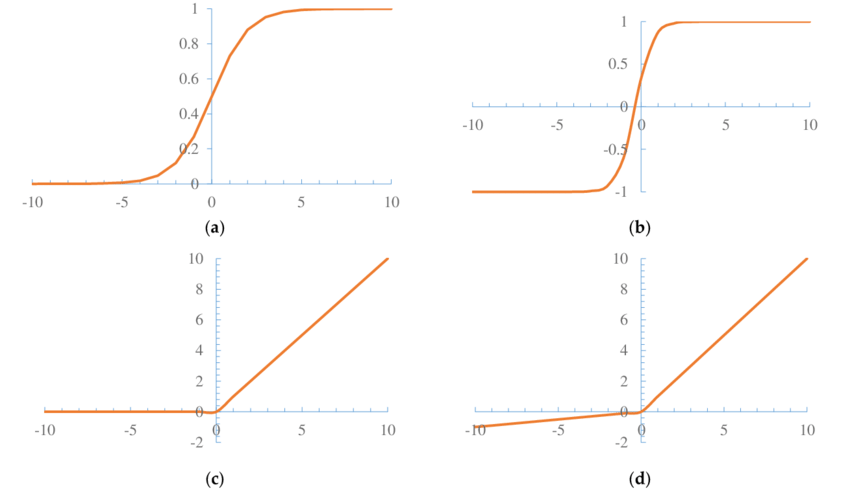
\includegraphics[width=1\columnwidth]{03-neural-networks-in-tumor-detection/figures/nonlinear-activation-functions.png}}
    \caption{Nonlinear activation functions \textbf{(a)} Sigmoid, \textbf{(b)} Tanh, \textbf{(c)} ReLU, and \textbf{(d)} Leaky ReLU \cite{yang2018modified}}
    \label{figure:nonlinear-activation-functions}
\end{figure}

        The non-linear activation functions more preferred over the linear activation functions.
        It helps to the model to generalize or adapt data. They are basically grouped by their curves and ranges.
        Commonly used activation functions such as Softmax, Sigmoid, Tanh, ReLU, Leaky ReLU and PReLU are examined in this section.

        \paragraph{Sigmoid} functions are smooth and continuously differentiable which means the slope of the Sigmoids can be found for any two points.
            The Sigmoids are monotonic but their derivatives are not.
            In Sigmoids, the Y values tend to respond very less to changes in X as it can be seen in Equation \eqref{sigmoid}.
            It means that small changes in the X values will cause larger changes in the Y values in this range.
            So the purpose of this function is to try to keep the Y values to the extremes.
            This is helpful when classifying the values into a particular class.
            If they are compared to linear functions, the outputs are always stay in a fixed range (0,1) unlike the linear functions whose outputs can be in the range of infinity.
            It is clearly understood that the Sigmoid function produces positive values for all the points and it is not symmetric around the origin.

            \begin{equation}
                h_ \theta (x) =  \frac{\mathrm{1} }{\mathrm{1} + e^- \theta^Tx } \label{sigmoid} \\
            \end{equation}

        \paragraph{Softmax} is a Sigmoid function derivative which gives remarkable results in multi variant image classification.

            \begin{equation}
                y_i(z_i) = \frac{e^{z_i}}{ \sum\nolimits_{k=1}^{k}{e^{z_k}} } \label{softmax} \\
            \end{equation}

        \paragraph{Tanh} function is an activation function which is a scaled version of the Sigmoid function.
            The difference between the Sigmoid and the Tanh is that the Tanh is symmetric over the origin whereas the Sigmoid is not symmetric, so the range of the Tanh is between -1 and 1.
            Continuity and differantiability of the Tanh is similiar to the Sigmoid, it is continuous and differentiable.

            \begin{equation}
                tanh(x) = \frac{2}{(1+e^(-2x)) -1} \label{tanh} \\
            \end{equation}

            It is preferred to Softmax if there are no more than two classes in a classification problem.
            The advantage is that the negative inputs will be mapped strongly negative and the zero inputs will be mapped near zero in the Tanh graph.

        \paragraph{Rectified Linear Unit (ReLU)}is an activation function which is non-linear and the most widely used activation function while designing neural networks today.

            \begin{equation}
                  f(x) = x^+ = \max(0, x) \label{relu} \\
            \end{equation}

            The non-linearity makes backpropagate the errors and have multiple layers of neurons being activated by ReLU function easy.
            ReLU does not activate the all neurons at once
            As it can be seen in Equation \eqref{relu}, the neuron does not activated if the input is not positive.
            This may cause the dead neurons problem which is the main problem of ReLU.
            In this activation function, only a few neurons are activated at a time. This makes the network sparse means efficient and easy for computation.

        \paragraph{Leaky ReLU} function is an improved version of the ReLU function.
            The gradient which is \emph{0} for \emph{x < 0} in ReLU make the neurons die for activations in that region.
            Leaky ReLU is focused on solving the dead neurons problem.
            The function is defined as a small linear component of \emph{x}.

            \begin{equation}
                 f(x) = \begin{cases} x &
                    \text{if } x > 0, \\
                    0.01x & \text{otherwise}.
                 \end{cases}\\
            \end{equation}

        \paragraph{PReLU} which is also known as Parameterised ReLU is very similar to the Leaky ReLU.

            \begin{equation}
                 f(x) = \begin{cases}
                    x & \text{if } x > 0, \\
                    a x & \text{otherwise}.
                \end{cases}
            \end{equation}

            In this context, \emph{a} is a trainable parameter which its values is learnt the network for faster and more optimum convergence.
            PReLU is preferred when Leaky ReLU fails to passing the relevant information to the next layer with solving the dead neurons problem.

    \subsection{Loss Functions}

        Loss function which is also called cost function evaluates the penalty between the ground truth label and the prediction during the training process to detect how well neural network models the dataset.
        The output of the loss function is inversely proportional to the success of the model, meanly higher numbers in the output are the sign of the unsuccessful model.
        Loss function is used the error which is calculated during backpropagation to update the weights in the negative direction of its derivative.

        In this section, some of the commonly used loss functions for image segmentation such as weighted cross entropy, balanced cross entropy, and Dice loss are examined.

        \paragraph{Weighted Cross Entropy (WCE)} weights the classes based on the fraction of the respective class in the total dataset as it can be seen in Equation \eqref{wce-loss} which is the definition of WCE for prediction \emph{p} and label $\hat{p}$.
            Thus, a class with a low fraction of the pixels in the dataset will get a high weighting. This is particularly interesting when the dataset contains unbalanced classes.

            \begin{equation}
                \text{WCE}\left(p, \hat{p}\right) = -\left(\beta p \log\left(\hat{p}\right) + (1-p) \log\left(1 - \hat{p}\right)\right) \label{wce-loss} \\
            \end{equation}

            $\beta \emph{> 1}$ should be setted to reduce the false negative rates while $\beta \emph{< 1}$ should be setted to reduce the false positive rates.

        \paragraph{Balanced Cross Entropy (BCE)} another variant of cross entropy which differs from WCE is that weighting the negative examples also.

            \begin{equation}
                \text{BCE}\left(p, \hat{p}\right) = -\left(\beta p \log\left(\hat{p}\right) + (1 - \beta)(1-p) \log\left(1 - \hat{p}\right)\right) \label{bce-loss} \\
            \end{equation}

        \paragraph{Dice Loss} \mbox{}\\

            The values of Dice ranges from zero to one, and high value means high similarity between the segmentations.
            For two overlapping regions, the Dice is defined as two times the intersection over the union.
            Dice loss is defined in Equation \eqref{dice-loss} for prediction \emph{p} and label $\hat{p}$.

            \begin{equation}
                \text{DL}\left(p, \hat{p}\right) = 1 - \frac{2\sum p_{h,w}\hat{p}_{h,w}}{\sum p_{h,w} + \sum \hat{p}_{h,w}} \label{dice-loss} \\
            \end{equation}
